\chapter{CVS, Gmake and the Bmad Distribution}
\label{c:cvs_gmake}
\index{CVS}
\index{Gmake}

\index{Tao}
The Bmad distribution is stored in a \cvs repository. \cvs
(Concurrent Versions System) is a widely used system for maintaining
documents. That is, by using \cvs one can keep track of past
versions of documents, can keep a log of who, when, and why changes
occurred, can coordinate multiple people working on the same document,
etc.  Documentation on \cvs can be obtained on Unix or Linux by
using the \vn{man cvs} command. In the case of \bmad, most of the
documents are code files but the \bmad and \tao documentation is
also maintained under \cvs.

\index{GNU}
\vn{Gmake} is the \vn{GNU} version of the \vn{make} system. Gmake is a
system whereby, after changes to program or library files are made,
only those files that need recompiling are recompiled. Considering the
time it can take to compile this represents an enormous savings in
time. Actually \vn{gmake} is more general than this but for the
purposes of this discussion the interested reader is referred to the
\vn{Gmake} documentation which can be obtained on Unix or Linux by
using the \vn{man gmake} or \vn{man make} command.

\cvs and \vn{gmake} are very sophisticated systems and this
documentation only gives some of the basics to enable someone to
develop programs based upon \bmad.

%----------------------------------------------------------------------------
\section{Setting up CVS}
\label{s:cvs_setup}
\index{CVS!setup}

\index{CVS!repository}
A ``repository'' is the place where \cvs keeps the information
about the files (called ``sources'') it is maintaining. The repository
contains all the information to permit extracting previous versions of
the sources at any time based on either a symbolic revision tag, or a
date in the past.

You don't need to setup a \cvs repository for \bmad (it already
exists) but \cvs can, in general, be useful for projects of all
stripes from writing a book to maintaining code. Therefore, this
section gives a brief overview of how to setup your own \cvs
repository.

The \cvs repository is setup by creating a ``root'' directory
to hold it using the command
\begin{example}
  cvs -d <root_dir> init
\end{example}
\vn{<root_dir>} is the root directory name. \cvs will create
\vn{<root_dir>} and initialize it. \vn{<root_dir>} must be an
absolute pathname. For example:
\begin{example}
  cvs -d /home/dcs/cvs_root init
\end{example}

By first setting the \vn{CVSROOT} environmental variable one can avoid
the typing of \vn{-d <root_dir>} in this and other commands.
\vn{CVSROOT} is set with the command
\begin{example}
  setenv CVSROOT <root_dir> # tcsh
  export CVSROOT            # bash, needed if CVSROOT is not already defined
  CVSROOT=<root_dir>        # bash
\end{example}
When \cvs looks for the \cvs root directory it first looks for the
\vn{-d} option on the command line. If that is not present it looks
for a \vn{CVS} directory in the current working directory where it can
read the \vn{CVS/Root} file (see below). If this is not present \cvs
will look at the \vn{CVSROOT} environmental variable.

\begin{figure}[tb]
\begin{centering}
\includegraphics{cvs.eps}
\caption{A) Example Project before Importing to CVS. B) Project when checked--out.}
\end{centering}
\label{f:cvs}
\end{figure}

After creating the repository root directory, go to the directory that
holds the files you want maintained in \cvs. To import these files
into the \cvs repository use the command
\begin{example}
  cvs -d <root_dir> import -m "<comment>" <project_name> <vendor_tag> <release_tag>
\end{example}
Everything in the current directory and subdirectories will be put
into \cvs under the \vn{<project_name>} name.  \vn{<comment>} is the
comment string associated with the initial source
files. \vn{<vendor_tag>} and \vn{<release_tag>} are tags important
when there is branching. Branching is a way to effectively have
different repositories (the different branches) for the same
project. The subject of branching is beyond the scope of this writeup
and the reader can look at the \cvs man pages for more details.  An
example import is shown in Figure~\ref{f:cvs}A which shows the
directory tree for a directory called
\vn{original_dir}.  Making \vn{original_dir} your working
directory and using the command
\begin{example}
    cvs -d /home/dcs/cvs_root import -m "start here" mad garbage1 garbage2
\end{example}
imports the 4 files in \vn{original_dir} into the repository and
associates these with the name \vn{mad}. If you have more than one
project you can do multiple imports. Just use a different
\vn{<project_name>} for each import.

%----------------------------------------------------------------------------
\section{Using CVS}
\label{s:cvs_use}
\index{CVS}

After you have imported files to a \cvs repository, or if you are using
an existing repository, you can check out a local copy of the files in the
repository by using the command
\begin{example}
  cvs -d <root_dir> co <project_name>
\end{example}
This will make a subdirectory \vn{<project_name>} with everything in it.
Following the example of the previous section the command
\begin{example}
  cvs -d /home/dcs/cvs_root co mad
\end{example}
will create a \vn{mad} directory in your working directory as shown in
Figure~\ref{f:cvs}B. The name \vn{mad} has replaced the name
\vn{original_dir} as the root of the files. There has also been added
new directories named \vn{CVS}. At this initial stage each \cvs
directory has three files called \vn{Entries}, \vn{Repository} and
\vn{Root}. The \vn{Entries} files give the files and directories that
\cvs that mirror files and directories in the \cvs repository. For
example the file \vn{bmad/CVS/Entries} contains the lines:
\begin{example}
  /file1/1.1.1.1/Thu Mar 24 20:27:07 2005//
  /file2/1.1.1.1/Thu Mar 24 20:27:07 2005//
  D/this_dir////
\end{example}
This shows that the checked out \vn{file1} file has version 1.1.1.1
and \vn{this_dir} is the associated directory. The \vn{Repository} files
give the directory path. Thus the file \vn{mad/this_dir/CVS/Repository}
contains the single line:
\begin{example}
  /mad/this_dir
\end{example}
Finally the \vn{Root} files just contain the directory of the
repository which in this case is
\begin{example}
  /home/dcs/cvs_root
\end{example}
The files in the \cvs directories should never be touched since
this could cause \cvs to misbehave. 

Sometimes there can be a problem with file permissions preventing a
check--out (or a check--in as explained below). If this happens there
will be an explicit error message as to what file in the repository
cannot be read and the solution is to use the \vn{chmod} command to
set the permission correctly.

You are fee to modify the files you have checked out from the
repository. The files in the repository will not be affected by this.
At some point you may want to put your modified files into the
repository. The command to check--in the files is
\begin{example}
  cvs ci -m <comment> <file_or_dir_name>
\end{example}
If \vn{<file_or_dir_name>} is a directory then \cvs will check--in all
files of that directory and any sub--directories under it. If
\vn{<file_or_dir_name>} is not present then the current working
directory is used. \vn{<comment>} is a comment associated with the
modified files. If you omit the \vn{-m <comment>} option then \cvs
will pop up an emacs window for you to type a comment in.
For example, if \vn{mad/file1} has been modified
and if \vn{mad} is the current directory, the command
\begin{example}
  cvs ci -m "My First Revision"
\end{example}
will check-in \vn{file1} to the repository. The information printed to
the terminal when this command is executed looks like:
\begin{example}
  cvs commit: Examining mad
  cvs commit: Examining mad/this_dir
  Checking in mad/file1;
  /home/dcs/cvs_root/mad/file1,v  <--  file1
  new revision: 1.2; previous revision: 1.1
\end{example}
The new version is labeled \vn{1.2} which can be seen by using the command
\begin{example}
  cvs log -r <version> <file>
\end{example}
The \vn{-r <version>} tells \cvs what version you want to see the log
of. If \vn{<version>} is not present then the latest is taken. If
\vn{-r <version>} is not present then the entire log for \vn{file} is
given. For example, using the command 
\begin{example}
  cvs log file1} 
\end{example}
will produce:
\begin{example}
  RCS file: /home/dcs/dcs/temp/cvsroot/mad/file1,v
  Working file: file1
  head: 1.2
  branch:
  locks: strict
  access list:
  symbolic names:
          garbage2: 1.1.1.1
          garbage1: 1.1.1
  keyword substitution: kv
  total revisions: 3;     selected revisions: 3
  description:
  ----------------------------
  revision 1.2
  date: 2005/03/25 01:02:15;  author: dcs;  state: Exp;  lines: +1 -0
  My First Revision
  ----------------------------
  revision 1.1
  date: 2005/03/24 20:27:07;  author: dcs;  state: Exp;
  branches:  1.1.1;
  Initial revision
  ----------------------------
  revision 1.1.1.1
  date: 2005/03/24 20:27:07;  author: dcs;  state: Exp;  lines: +0 -0
  start here
  =============================================================================
\end{example}
The initial version was labeled \vn{1.1.1.1}. Since branching is not
being used here \cvs automatically made another version labeled
\vn{1.1} but this did not do anything with the file contents. When the
local \vn{file1} was revised and the \vn{cvs ci file1} command was
issued the new version was labeled \vn{1.2}. latter versions will be
labeled \vn{1.$n$} where $n$ will be increased by 1 for each new
version. Notice that each file has a separate revision number so that,
at any point in time, the latest revision numbers for the files will
not, in general, all be the same. The \vn{start here} line in the log
under revision 1.1.1.1 comes from the \vn{-m} comment in the \vn{cvs
import} command (see the example in the previous section) used to
create the \vn{mad} repository. The \vn{Initial revision} line in the
log is generated by \cvs. The \vn{My First Revision} line in the log
comes from the \vn{cvs ci} command.  The \vn{lines: +1 -0} under
\vn{revision 1.2} in the log show that 1 line has been added and no
lines deleted in this revision from the last.

If you want to know what files have been modified from what is in the
repository you use the command
\begin{example}
  cvs diff <file_name>
\end{example}
The output of this command is similar to the Unix \vn{diff} command.
For example, if the version of \vn{file1} in the repository has the lines
\begin{example}
  Original 1
  Original 2
\end{example}
and the local \vn{file1} is modified so that these lines are replaced by
\begin{example}
  New A
  New B
  New C
\end{example}
then the diff command will produce the output
\begin{example}
  Index: file1
  ===================================================================
  RCS file: /home/dcs/cvs_root/mad/file1,v
  retrieving revision 1.2
  diff -r1.2 file1
  37,38c37,39
  < Original 1
  < Original 2
  ---
  > New A
  > New B
  > New C
\end{example}
The \vn{diff -r1.2 file1} shows that the difference is between version
1.2 of \vn{file1} in the repository and the local \vn{file1} The
\vn{37,38c37,39} descriptor means that in the repository version of
\vn{file1} the lines \vn{Original 1} and \vn{original 2} where at
lines 37 through 39. In the new file the lines \vn{New A} through
\vn{New C} are at lines 37 through 39. If multiple sections of a file
are modified then the \vn{diff} output will contain multiple blocks of
a descriptor followed by the lines from the repository file that were
modified or deleted followed by the corresponding lines from the local
file.  If the descriptor contains a \vn{d} then this means that the
local file has had lines deleted from it. If the descriptor has a
\vn{a} then the local file has had lines added to it. To look at the
difference between two versions in the repository use the \vn{-r
<version>} option. In the current example, to see the difference
between versions 1.1 and the latest (1.2) of \vn{file1} the command
would be
\begin{example}
  cvs diff -r1.1 -r file1
\end{example}

A \vn{cvs co}, as discussed above, will make a local copy of the latest
version of each file of a project. This is normally what is wanted but
in some cases what is needed are the files from a certain point. For
example, you might want the files for a date just before some
revisions where made to check against the latest version. 

The \vn{cvs co} command has an option to do this but finding what date
is needed could be problematical. A way around this is to tag all
the files in the project with a given tag string. \cvs can then
retrieve the files associated with a given tag string. Tag the
latest versions of the files in the repository uses the command
\begin{example}
  cvs -d <root_dir> rtag <tag> <project_or_file_name>
\end{example}
Tags must not contain any spaces. For example, the command
\begin{example}
  cvs rtag tag_number_1 mad
\end{example}
will tag all the \vn{mad} project files. [It is always assumed in the
examples that the working directory is \vn{mad} so the \vn{-d} option
does not have to be used.] To see the tags associated with a file use
the command
\begin{example}
  cvs status -v <file>
\end{example}
Thus if the \vn{mad} project has been tagged as above the command
\begin{example}
  cvs status -v file1
\end{example}
Produces
\begin{example}
  =================================================================
  File: file1             Status: Up-to-date
  
     Working revision:    1.2     Fri Mar 25 01:02:15 2005             
     Repository revision: 1.2     /home/dcs/cvs_root/mad/file1,v
     Sticky Tag:          (none)
     Sticky Date:         (none)
     Sticky Options:      (none)
  
     Existing Tags:
          tag_number_1                    (revision: 1.2)
          garbage2                        (revision: 1.1.1.1)
          garbage1                        (branch: 1.1.1)
\end{example}

To check out the files associated with a certain tag use the command
\begin{example}
  cvs -d <root_dir> co -r <tag> <project_or_file_name>
\end{example}
Note that this command can also be used to check--out files with a
given version number. by using the version number in place of
\vn{<tag>}.

As the project develops files will be added and other files will be
deleted. The command to add a file to cvs is
\begin{example}
  cvs add <file>
\end{example}
The file must already exist. \cvs will not actually add the file to
the repository until a \vn{cvs ci} is issued. For example, if a file
\vn{new_file} is added to the \vn{this_dir} directory then it is added
with the commands
\begin{example}
  cvs add this_dir/new_file
  cvs ci
\end{example}
[Again it is assumed that \vn{mad} is the working directory.] A common
mistake here is to forget to a \vn{cvs add}. \vn{cvs ci} will not warn
you about added files that are not in the repository. To see the
status of all the files in your area use the command
\begin{example}
  cvs -n update
\end{example}
For example, if no \vn{cvs add} had been done for \vn{new_file} then
the \vn{cvs -n update} command would produce
\begin{example}
  cvs update: Updating .
  cvs update: Updating this_dir
  ? this_dir/new_file
\end{example}
The \vn{?} indicates that \vn{new_file} is not in the repository. The
\vn{-n} option is important in that it prevents \vn{cvs} from actually
updating the repository (see below). Notice that having a local file
with no corresponding repository file is not necessarily an error
since there may be local files that are not meant to be in the
repository.

The command to delete a file is
\begin{example}
  cvs delete <file>
\end{example}
The file must have been deleted before you run this command. The file
will not actually be deleted from the repository until you do a
\vn{cvs ci}.

Multiple people may check--out the same project and make revisions
(and one person may check--out multiple copies of a project in
multiple areas). The command to update your local copy of a project
after someone else (or you in another local copy) has made changes to
the repository is
\begin{example}
  cvs update
\end{example}
As \cvs updates you local files it prints information on what it is
doing. For example, if someone else has added the file \vn{other_file}
to the \vn{this_dir} directory then a \vn{cvs update} will print
\begin{example}
  cvs update: Updating .
  cvs update: Updating this_dir
  U other_file
\end{example}
The letter before a file name indicates the status:
\begin{example}
  U -- The local file was brought up--to--date
  A -- The local file is on the list of files to be added to the repository
          at the next cvs ci.
  R -- The file is on the list of files to be removed from the repository
          at the next cvs ci.
  M -- The local file has been modified since it was checked out. 
          Nothing is done to it.
  C -- A conflict: You have modified the local file while the same file
          from another source has been checked into the repository.
          The files will be merged.
  ? -- The local file has no corresponding file in the repository.
\end{example}
In the case of a conflict \cvs will merge the repository file with
your local file. It does this by taking considering the version of the
file that you checked out from the repository. Call this the \vn{base}
version. \cvs then looks at the difference blocks for 1) the local
file and the base version (call this a \vn{local} difference block)
and 2) the latest version in the repository and the base version (call
this a \vn{repository} difference block). If a \vn{repository}
difference block does not overlap any of the \vn{local} difference
blocks the difference block is used to modify the local file. If a
\vn{repository} difference block does overlap a \vn{local} difference
block then the merged file will contain both blocks and it is up to
you to edit the file and to resolve the conflict. The important point
here is that \cvs {\it never} deletes any changes you have made. You
can never loose work you have done my updating. When there is a
conflict the local file will have a section that looks like
\begin{example}
  This part of the file was not modified.
  ... etc ...
  <<<<<<< file1
  This part of the file was locally modified
  ... etc ...
  =======
  This part of the file was modified by someone else
  ... etc ...
  >>>>>>> 1.3
  ... etc ...
\end{example}
The \vn{<<<<<<< file1}, \vn{=======}, and \vn{>>>>>>> 1.3} lines are
added by \cvs to delineate the text coming from the local
modification from the text from the repository modification.

If there is a conflict between a file in the repository and a local
file then \cvs will not let you do a \vn{cvs ci} on the project. What
needs to be done first is a \vn{cvs update} after which you can do a
\vn{cvs ci}. If you want to just check--in one file even when there is
a conflict with another file you can do a \vn{cvs ci <file>} to just
check in that file. You can never check-in a local file that has a
conflict with the repository.

The repository can also be accessed remotely (something akin to ftp)
by setting two environmental variables on the remote system
\begin{example}
  setenv CVS_RSH ssh
  setenv CVSROOT :ext:<user>@<root_dir>
\end{example}
In this case \vn{<root_dir>} must contain the computer name. For example:
\begin{example}
  setenv CVS_RSH ssh
  setenv CVSROOT :ext:dcs@cesr66.lepp.cornell.edu/home/dcs/cvs_root
\end{example}
You will be asked to supply a password but other than that will
behave exactly like the repository was on the local disk.


%----------------------------------------------------------------------------
\Section{Using CVS with Bmad}

The \cvs repository for \bmad contains \bmad and the associated
libraries (\sref{s:libs}). Periodically all the libraries are checked
out and compiled. This is called a \vn{release}. Typically the release
root directory is named after the creation date. For example one release is:
\begin{example}
  /home/cesrulib/cesr_libs/OSF1_alpha/cesr_2005_0320_d
\end{example}
This is a release for the OSF True64 computers built on March 20,
2005. There needs to be different releases for different platforms
since the compiled binary files will be different. At this time there
are actually different releases on Linux for the two compilers (from
Lahey--Fujitsu and Intel) in use since the binary files from these
compilers are not compatible. It is important that if you are
developing on different platforms or are developing with different
compilers that you keep your binaries separate as well.

The latest release has a soft link named \vn{devel}. There is
also a \vn{current} soft link that
points to the last "stable" release that is felt to be (relatively)
bug free. The advantage to using the \vn{devel} version over
\vn{current} is that you get the latest bug fixes (if any). The
disadvantage is that it might not be as stable. Typically people use
the \vn{devel} release.

To initialize for \bmad, the \vn{CESRLIB} environmental variable needs
to be set to the desired release root directory and the appropriate
command file must be run. This command file is different for the
\vn{bash} and \vn{tcsh} shells. For example, with \vn{tcsh}, to run
the devel release put the following lines in your \vn{.login} file:
\begin{example}
  setenv CESRLIB devel
  source /home/cesrulib/bin/cesrdef
\end{example}
For \vn{bash} use
\begin{example}
    CESRLIB=devel
    . /home/cesrulib/bin/cesrdefs
\end{example}
Other releases can be used by setting \vn{CESRLIB} appropriately. To
see the names of all the releases look at the directory appropriate
for the compiler and platform which at present are
\begin{example}
  /home/cesrulib/cesr_libs/Linux_alpha       # Linux    Lahey
  /home/cesrulib/cesr_libs/Linux_i686        # Linux    Intel
  /home/cesrulib/cesr_libs/OSF1_alpha        # OSF      Intel
  /home/cesrulib/cesr_libs/CYGWIN_NT_i686    # Windows  Intel
  /home/cesrulib/cesr_libs/VMS_alpha         # VMS      HP
\end{example}

To see the logicals that are setup by the \vn{cesrdef(s)} command file
use the following command:
\begin{example}
  printenv | grep CESR
\end{example}
This might produce
\begin{example}
  CESRLIB=devel
  CESR_PLATFORM=OSF1_alpha
  CESR_BASE=/home/cesrulib/cesr_libs/OSF1_alpha
  CESR_CURRENT=/home/cesrulib/cesr_libs/OSF1_alpha/current
  CESR_DEVEL=/home/cesrulib/cesr_libs/OSF1_alpha/devel
  CESR_DOC=/home/cesrulib/cesr_libs/doc
  CESR_CVSROOT=/home/cesrulib/cesr_libs/cvsroot
  CESR_REL=/home/cesrulib/cesr_libs/OSF1_alpha/devel
  CESR_CONFIG=/home/cesrulib/cesr_libs/OSF1_alpha/devel/config
  CESR_CVSSRC=/home/cesrulib/cesr_libs/OSF1_alpha/devel/cvssrc
  CESR_EXE=/home/cesrulib/cesr_libs/OSF1_alpha/devel/bin
  CESR_GMAKE=/home/cesrulib/cesr_libs/OSF1_alpha/devel/Gmake
  CESR_LIB=/home/cesrulib/cesr_libs/OSF1_alpha/devel/lib
  CESR_MOD=/home/cesrulib/cesr_libs/OSF1_alpha/devel/modules
  CESR_RUN=/home/cesrulib/cesr_libs/OSF1_alpha/devel/run
  CESR_UTIL=/home/cesrulib/cesr_libs/OSF1_alpha/devel/util
  CESR_INC=/home/cesrulib/cesr_libs/OSF1_alpha/devel/cvssrc/include
  CESR_PKG=/home/cesrulib/cesr_libs/OSF1_alpha/devel/packages
  CESR_CONST=/home/cesrulib/constants
\end{example}

The source code for the local libraries (\vn{Bmad}, \vn{cesr_utils},
\vn{recipes_f-90_LEPP}, and \vn{dcslib}) is in \vn{CESR_CVSSRC}. The
source code for the outside libraries (\vn{forest}, \vn{recipes},
\vn{PGPLOT}, and \vn{xsif}) is in \vn{CESR_PKG}. The
\vn{recipes_f-90_LEPP} library is the specially modified version of
Numerical Recipes (\sref{s:libs}) that can handle either single or
double precision reals. This is not to be confused with the original
single precision version (which is never compiled) \vn{recipes_f-90}
which is in \vn{CESR_PKG}. 

A web based viewer has been setup for \bmad. It can be accessed at
\begin{example}
  http://www.lns.cornell.edu/~cesrulib
\end{example}

Some programs are also maintained in the the \cvs repository. some of
these are compiled and linked with a release. The executables are in
\vn{CESR_BIN}. The most notable is \vn{bmadz} which is the CESR
storage ring lattice design program.

If you just link against a release you don't need to check--out and
compile any of the \bmad source code. If you do need to do this the
next section will explain how this is done.

For people outside Wilson Laboratory who need a local copy of \bmad
there are what are called \vn{distributions}. A \vn{distribution} is
made by checking out the \bmad distribution and taring it into one
file for portability. \vn{Distributions} may be obtained from the
\bmad web page (\sref{s:libs}).

%----------------------------------------------------------------------------
\section{Compiling and Linking Bmad Programs}
\label{s:compile}

\begin{figure}[tb]
\begin{centering}
\includegraphics{devel_dir.eps}
\caption{Standard Directory Structure for Bmad Programs.}
\end{centering}
\label{f:devel_dir}
\end{figure}

To facilitate the automatic compiling and linking of programs there
is a standard directory structure that is used with \bmad as shown in
Figure~\ref{f:devel_dir}. \vn{<devel_dir>} is the root development
directory (names in braces \vn{<..>} means that you choose the name,
names without braces means that the name is standardized). In
Figure~\ref{f:devel_dir} \vn{<program1_dir>} and \vn{<program2_dir>}
are directories for developing programs. Although only two program
directories are shown, there is no limit as to their number. Code
files can be put in a program directory or in sub--directories. The
\vn{lib} directory of for compiled libraries, the \vn{modules}
directory is for compiled Fortran modules, and the \vn{bin} directory
is for executable files. There can also be local copies of the
\vn{bmad} library and it subsidiary libraries (\sref{s:libs}).

\index{Gmake}
A program directory will always have a \vn{Makefile} file that is used
by \vn{gmake} to compile and link programs. Any local libraries will
also have their own \vn{Makefile} files. Program makefiles are
different from library makefiles and even among program makefiles no
two makefiles are necessarily the same. More will be said of this
later.

Any given program directory can have one or multiple programs within
it. If it has only one program then to compile and link the program
use the command
\begin{example}
  gmake
\end{example}
the default \vn{gmake} behavior in this case is to name the executable
file after the program directory name and not the program file
name. For example, in Figure~\ref{f:devel_dir}, the executable made
from \vn{test.f90} in \vn{<program2_dir>} is
\vn{bin/<program2_dir>}. There are actually two different executables:
A \vn{production} executable and a \vn{debug} one. The \vn{debug}
executable has a \vn{_g} appended to the name so in this example its
name is \vn{bin/<program2_dir>_g}.  The production executable will run
much faster than the debug version (roughly a factor of 3 or so). The
debug version, however, can be used with a debug program to examine
the program as it is running.  The debug version of the program, just
like the production version, can be run without a debugger and this is
sometimes useful since the debug version will catch errors such as an
array index out of bounds that the production version would not.

Along with the executables, \vn{gmake} will make a \vn{.map} file for
each executable which shows where each routine that is part of the
program came from. The \vn{.map} files are are sometimes helpful in
debugging a program. For example, \vn{bin/<program2_dir>_g.map} is the
map file associated with \vn{bin/<program2_dir>_g}.

To save time, if only the \vn{production} executable is needed, the command
\begin{example}
  gmake production
\end{example}
can be used. To create only the debug version use
\begin{example}
  gmake debug
\end{example}
If there is more than one program in a program directory then the
\vn{gmake} syntax is
\begin{example}
  gmake MAIN_FILE=<program_file_name>
\end{example}
In this case the executable file will be named after the program file
name.

\vn{gmake} tries to cut compile and link time by only compiling and/or
linking when file are "out-of-date". Thus \vn{gmake} will only relink
the executable if the creation date of the executable is prior to the
creation dates of the object files that are linked. The dependency
rules that \vn{gmake} used to decide if one file is dependent upon
another file is kept in a \vn{.depend} directory in a program
directory. Sometimes \vn{gmake} can become confused (say if a local
library is deleted) and if this happens the best way to reset things
is via the command
\begin{example}
  gmake clean
\end{example}
This removes the executables, object files and \vn{.depend} directory.

The standard debug program is called \vn{totalview}. \vn{totalview} is
put out by a company called Etnus and documentation on totalview can
be obtained from the web at
\begin{example}
  http://www.etnus.com
\end{example}

Local copies of \bmad and/or its subsidiary libraries are only
generally only needed in special circumstances. Problems can arise
with local libraries if they are not keep up-to-date with the
repository versions. For this reason it is best to remove local
libraries if they are no longer needed. The command for this is
\begin{example}
  gmake clean
\end{example}
Just removing the library code directory is not enough since modules
in the \vn{modules} directory and the library itself in the \vn{lib}
directory will remain. When compiling libraries it must be remembered
that there is a definite order to the compilation. This is due to the
fact that since Fortran modules are compiled, if a library has a
module that is used by a file in another library, the first library
must be compiled first. The order of libraries is
\begin{example}
  bmad
  dcslib
  cesr_utils, forest, recipes_f-90_LEPP, XSIF 
\end{example}
The bottom most libraries must be compiled first.
